\chapter{Introduction}

This initial parts of this chapter will mostly serve as a historical overview of the field of particle physics, with an emphasis on the development of the \textbf{Standard Model}--the theory that describes all of the fundamental\footnote{As of the year 2023, but reading this chapter will hopefully illustrate why this may be subject to change in the future.} particles and the way in which they interact with each other. 

As this thesis is focused nearly entirely on the strong nuclear force, the remaining parts of the chapter will provide a thorough discussion of Quantum ChromoDynamics (QCD), which is the component of the Standard Model which describes the interactions between \textbf{quarks} and \textbf{gluons}--the consituent particles of the more familiar protons and neutrons. Unfortunately, QCD is enormously complicated and the full theory is not yet fully understood. While this may be disheartening for theorists, it is a boon for experimentalists as it provides a wealth of opportunities to probe the theory in regimes where it is both understood and not understood. 

To this end, the remainder of this chapter will focus on the ways in which QCD can be investigated using heavy-ion collisions, with an emphasis on the \textbf{Quark-Gluon Plasma} (QGP)--a novel state of nuclear matter that QCD predicts should exist at the extreme temperatures and densities that are achieved in these collisions. The experimental signatures of QGP formation will also be discussed, with a particular focus on \textbf{strangeness enhancement}--the phenomenon where the production of strange quarks is enhanced in heavy-ion collisions relative to proton-proton collisions. 

\section{What is fundamental?}
The answer to the question ``What are the fundamental building blocks of our universe?'' has changed drastically over the course of human history. The idea that all matter is composed of smaller, uncuttable pieces has been around since 5th century BCE when Greek philosophers Democritus and Leucippus first introduced the concept of an atom~\cite{GreekAtom}. While this idea was mostly motivated by philosophical reasoning, it was later adopted by the English scientist John Dalton in the 19th century to explain the results of his chemical experiments, where he found that chemical elements always combined with each other by discrete units of mass~\cite{Dalton}. As scientists discovered more and more of these elements, the number of ``fundamental'' building blocks grew as well. By the late 1800s, over 70 unique chemical elements had been discovered, though they would often be grouped together due to similar chemical properties using what chemist Dimitri Mendeleev dubbed the \textit{periodic table of elements}~\cite{PeriodicTable}. An example of the periodic table from the time of Mendeleev can be seen in Figure~\ref{fig:periodic_table}. While this grouping was useful for chemists, it also served as a hint to physicists that perhaps these elements were not actually fundamental, but rather composed of even smaller pieces.

\begin{figure}[ht]
    \centering
    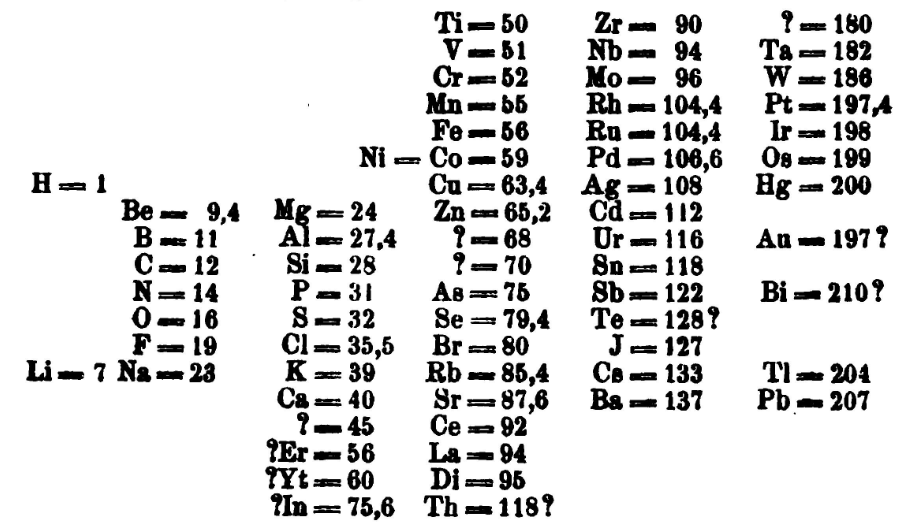
\includegraphics[width=0.7\textwidth]{figures/introduction/PeriodicTable.png}
    \caption{Dimitri Mendeleev's periodic table of elements from the late 1800s, taken from~\cite{MendeleevPaper}. The elements are grouped by similar chemical properties, and the gaps in the table are where Mendeleev predicted that new elements would be discovered.}
    \label{fig:periodic_table}
\end{figure}


Things changed quite a bit around the turn of the 20th century, with scientists like Rutherford and Chadwick determining that the supposedly indivisible atom was composed of even smaller sub-atomic particles, eventually named electrons, protons and neutrons~\cite{Electrons, Protons, Neutrons}. Thus the number of fundamental blocks of matter had decreased substantially from nearly 100 to just three, but only very briefly. Only months after the discovery of the neutron, the fundamental anti-particle of the electron--known as the positron--was discovered in 1932 by Carl Anderson~\cite{Positron}. In the next two decades, the number of known fundamental particles would skyrocket. In 1947, the muon was discovered~\cite{Muon}, followed by the discovery of a laundry list of particles that participate in the same interaction that holds oppositely charged protons together in the nucleus of an atom--the so-called \textbf{strong nuclear force}. These ``fundamental'' particles were collectively called \textbf{hadrons}, which were further separated into lighter and heavier categories dubbed \textbf{mesons} and \textbf{baryons}, respectively~\cite{MesonBaryon}. By the late 1960s, the number of known hadrons had grown to well over 100~\cite{ParticleDiscoveries}, which is ironically much higher than the number of ``fundamental'' chemical elements that were known to exist in the 1800s. 

In the same way that Mendeleev tried to group the elements by their similar chemical properties, physicists attempted to group the hadrons together based on their known sub-atomic properties at the time. The first successful attempt at such a grouping was the \textbf{Eightfold Way}, which was independently proposed by Murray Gell-Mann and Yuval Ne'eman in 1961~\cite{GellMann, Neeman}. When separating the hadrons into mesons and baryons, then further separating them by their spin, 


This classification scheme is depicted in Figure~\ref{fig:eightfold_way}.

and in 1961 Murray Gell-Mann and Yuval Ne'eman independently proposed a new way to organize the particles based on their various properties~\cite{GellMann, Neeman}. This new classification scheme, known as the \textbf{Eightfold Way}, is depicted in Figure~\ref{fig:eightfold_way}. 


\section{The Standard Model}
During this time, the theory that describes how light and matter interact (known as Quantum ElectroDynamics, or QED) was being developed by the likes of Feynman, Schwinger, Tomaga and Dyson~\cite{QEDFeymnan, QEDSchwinger, QEDTomaga, QEDDyson}. 

The notion that protons and neutrons were unbreakable was relatively short lived, as not even half a century later the deep inelastic scattering experiments performed by Kendall, Friedman and Taylor~\cite{Kendall, Friedman, Taylor} revealed that protons (and subsequently neutrons) were actually composed of even smaller particles, eventually dubbed ``partons''. \cite{Partons}.
This discovery was one of the largest contributing factors to the creation of the so-called Standard Model of particle physics, a theory which describes all of the fundamental particles and the way in which they interact with each other. A diagram of those fundamental particles can be seen in Figure~\ref{fig:standard_model}.
\begin{figure}
    \centering
    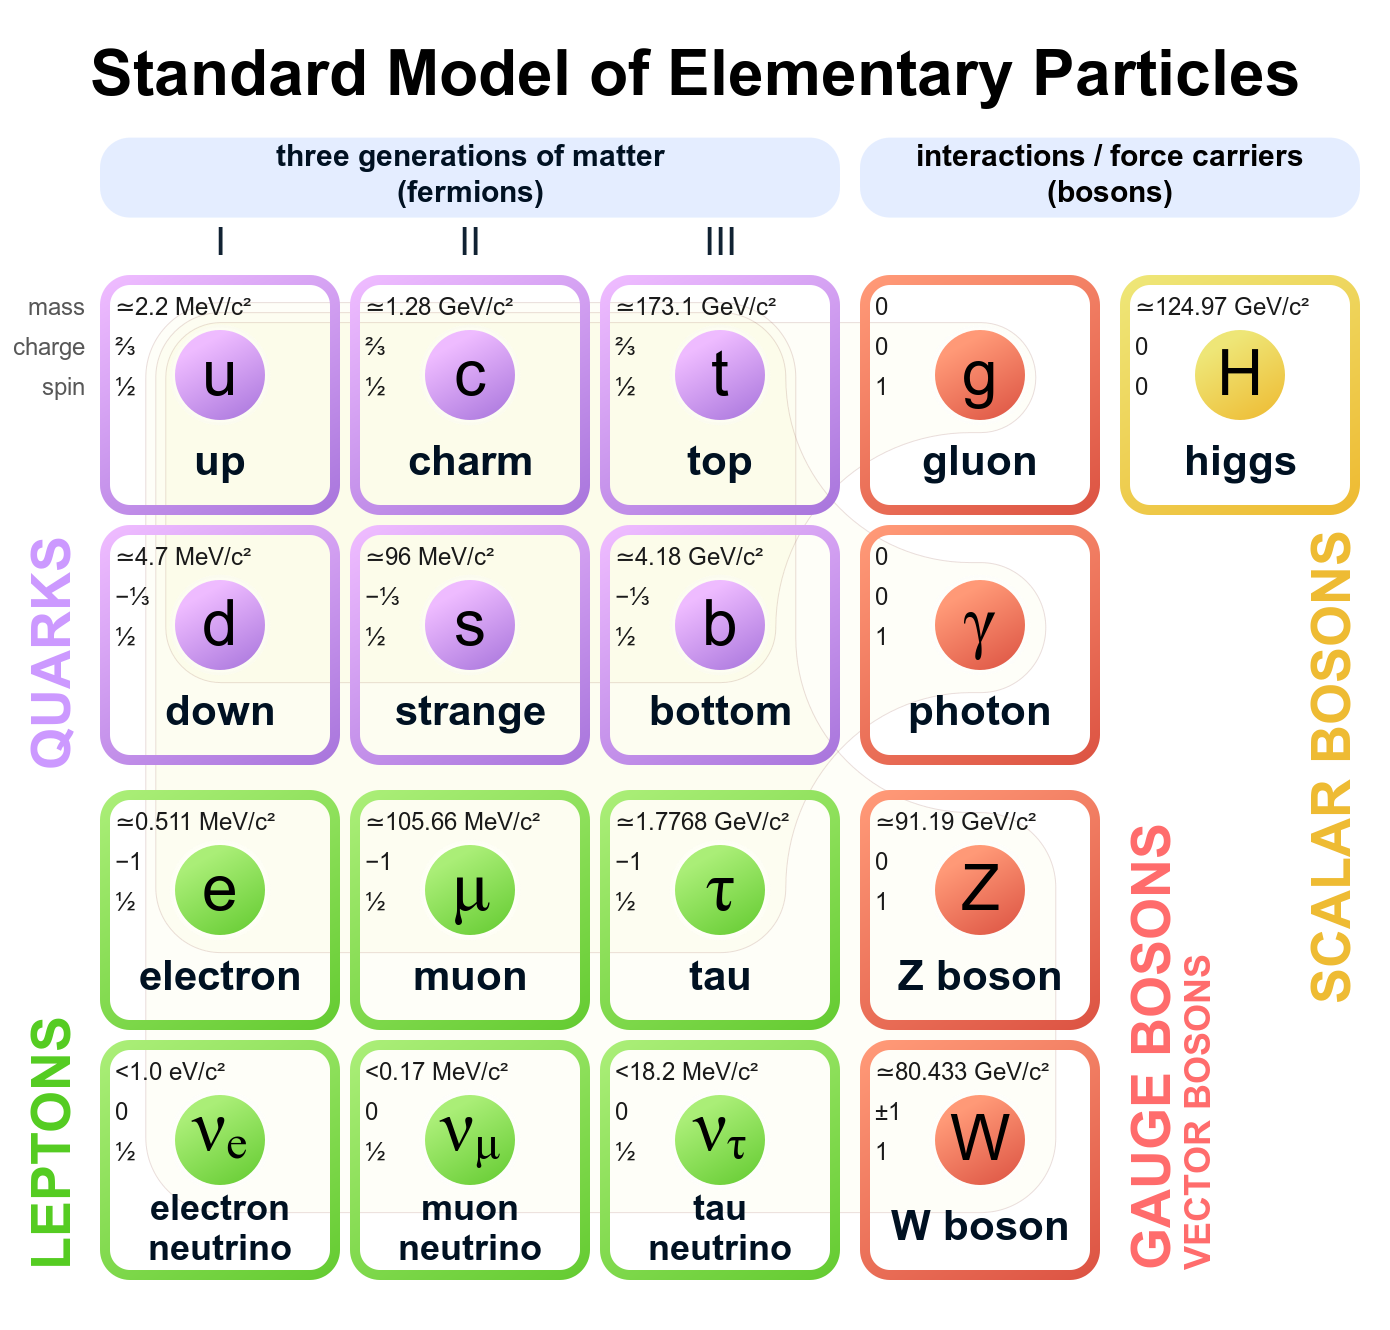
\includegraphics[scale=0.2]{figures/introduction/StandardModel.png}
    \caption{A diagram depicting the particles we currently believe are fundamental within the so-called ``Standard Model'' of particle physics.}
    \label{fig:standard_model}
\end{figure}
 It should be noted that all of the particles labeled as quarks and leptons -- collectively as ``fermions'' -- have corresponding anti-particles with opposite electric charge.
The equation that describes all of these particles and their interactions, often incorrectly\footnote[1]{It is ``incorrect'' because this is technically a Lagrangian density (i.e. Lagrangian per unit volume), but as it is usually integrated over all space the distinction is mostly irrelevant.} referred to as the ``Standard Model Lagrangian'', can be compactified into a relatively palatable form that can easily fit on a coffee cup like the one shown in Figure~\ref{fig:lagrangian_cup}.
\begin{figure}
    \centering
    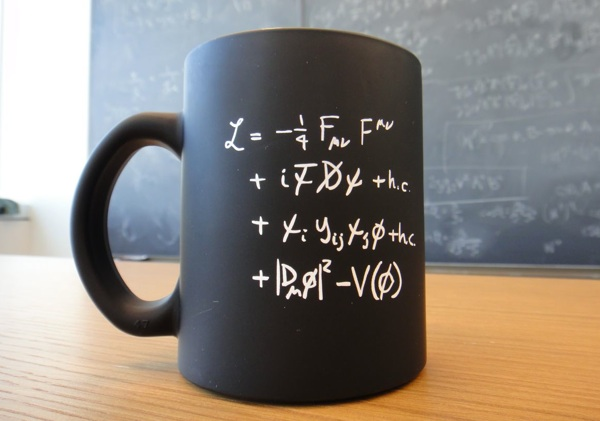
\includegraphics[scale=0.5]{figures/introduction/StandardModelCup.jpg}
    \caption{A coffee cup with the Standard Model Lagrangian density printed on its side. Please ignore the ``+ h.c.'' term following the $i\Bar{\psi}\slashed{D}\psi$, it is the result of a small lapse in judgement from the mug makers.}
    \label{fig:lagrangian_cup}
\end{figure}

While this equation may appear brief\footnote{Here ``brief'' is in the eye of the beholder, but certainly its brevity is misleading as even in the first line the $F_{\mu\nu}$ refers to three completely different gauge field tensors with their indices fully contracted...}, it can be used to completely describe three of the four fundamental forces of nature: 
\begin{enumerate}
    \item The Electromagnetic Force, which is responsible for the electrons pushing against each other to keep you from falling through your chair,
    \item The Weak Nuclear Force,  which is responsible for the initiating the nuclear fusion reactions that fuel our sun, and 
    \item The Strong Nuclear Force,  which is responsible for holding quarks and gluons together in bound stands known as hadrons, like the protons and neutrons that make up everyday matter.
\end{enumerate}
The only fundamental force missing from this list is the Gravitational Force, which is described by a completely separate set of equations\footnote{Specifically, the Einstein Field Equations, $G_{\mu\nu} + \Lambda g_{\mu\nu} = \kappa T_{\mu\nu}$, but this is the thesis of a particle physicist so gravity is taboo.}

Each of the three forces that are described within the Standard Model are mediated by different gauge bosons. For example, the electromagnetic force is mediated by the boson known as the photon, the weak nuclear force is mediated by the W and Z bosons, and the strong nuclear force is mediated by bosons known as gluons. 
In this thesis we will be primarily focusing on the Strong Nuclear Force, which acts solely on particles with color charge -- an intrinsic property of quarks and gluons. 
The ``color'' charges are red, green, and blue with antio

Even though each of the electromagnetic, weak and strong forces can be described using the Standard Model Lagrangian, the way in which they appear within the equation is not easy to determine.
For example, the electromagnetic force actually corresponds to line 1